\documentclass[11pt]{article}

\usepackage[margin=1in]{geometry}
\usepackage{amsmath,amssymb,amsthm}
\usepackage{hyperref}
\usepackage{float}
\usepackage{graphicx}
\usepackage{booktabs}
\usepackage{subcaption}
\usepackage{longtable}
\usepackage{fontspec}
\usepackage{tikz}
\usetikzlibrary{arrows.meta, backgrounds, calc, fit, positioning}

\tikzset{
  rtarrow/.style={->, >=Stealth, thick},
  rtlatent/.style={circle, draw, thick, minimum size=18pt, inner sep=1pt},
  rtobs/.style={rtlatent, fill=gray!20},
  rtconst/.style={rectangle, draw, thick, rounded corners, inner sep=2pt, minimum height=16pt},
  rtplate/.style={draw, rounded corners, dashed, inner sep=6pt},
}

\setmainfont{Times New Roman}
\setmonofont{Menlo}

\graphicspath{{./}{images/}{images/rt_pymc_multilevel_pooling_report/}{docs/models/}{docs/models/images/}{docs/models/images/rt_pymc_multilevel_pooling_report/}}

\setlength{\parindent}{0pt}
\setlength{\parskip}{0.7\baselineskip}

\title{Report: RT Regression Model (Hierarchical Ridge with Chemistry)}
\author{Bioinformatics Team}
\date{\today}

\begin{document}

\maketitle

\section{Introduction}

Retention time (RT) is a strong auxiliary signal for peak assignment. For a given compound, we compare an observed peak
RT to a model prediction and retain candidates that fall within an uncertainty window. This makes two properties
critical: accurate point predictions, and \emph{calibrated} uncertainty so that a nominal ``95\% window'' contains the
true RT about 95\% of the time.

In current production, the baseline is a bank of \textbf{supercategory-specific lasso regressions}. For each
\nolinkurl{species\_cluster} (supercategory / matrix), the baseline predicts RT from run covariates
(\texttt{IS*}/\texttt{RS*}/\texttt{ES\_\*}) using an $\ell_1$ penalty (lasso), and associates each prediction with a
hand-tuned window rather than a probabilistic predictive distribution. The implementation and model bundle live in the
Hippopotamus pipeline (\nolinkurl{external_repos/Hippopotamus}).

This baseline is useful, but it has limitations that matter for peak assignment:
\begin{itemize}
  \item \textbf{No partial pooling in the long tail.} Rare \nolinkurl{species} and sparse compound histories are fit
  largely independently, which can produce noisy predictions and inconsistent calibration when training support is low.
  \item \textbf{No chemistry-informed sharing across compounds.} Compound effects are treated as unrelated parameters,
  so the model cannot borrow strength across chemically similar compounds when compound history is sparse.
  \item \textbf{Heuristic uncertainty.} Window widths are not derived from a probabilistic model, so ``coverage'' is not
  a nominal probabilistic statement and is hard to tune systematically.
\end{itemize}

An $\ell_1$ (lasso) prior is also a poor default for our run covariates. \texttt{IS*} and \texttt{ES\_\*} predictors are
often strongly correlated because they capture overlapping aspects of run drift and instrument state. With correlated
predictors, lasso tends to select an arbitrary subset and set the rest to zero, making coefficients unstable across
retrains and creating brittle behavior on sparse groups. A ridge (Gaussian) prior is a better default here: it shrinks
correlated covariates smoothly instead of forcing hard selection, leading to more stable predictions and uncertainty
estimates.

We address these issues with a hierarchical Bayesian ridge model with chemistry-informed sharing. The model improves
long-tail stability via partial pooling across \texttt{species} nested in \texttt{species\_cluster}, regularizes
compound baselines via a chemistry-informed prior that shares information across compounds, and provides calibrated
uncertainty via an explicit predictive distribution.

For deployment, we export coefficient summaries (posterior means and variances), so scoring stays fast and simple:
compute a linear prediction from the run covariates and attach a Normal predictive interval, without running Bayesian
inference at runtime.

This report trains models for lib208 and lib209 and evaluates on the corresponding realtest splits, comparing against a
per-supercategory ridge baseline and the production lasso baseline. On these evaluations, the partial pooling model
improves RMSE relative to the ridge baseline while keeping coverage close to the nominal 95\% target.

\section{Methods: hierarchical ridge with chemistry}

This section describes the proposed model in full, starting from a high-level decomposition and then giving a complete
probabilistic specification (likelihood, priors, and inference).

\subsection{Data and notation}

Each RT observation row $i$ contains:
\begin{itemize}
  \item response $y_i$ (RT, minutes),
  \item run covariates $x_{i,j}$ for $j=1,\ldots,p$ from numeric \texttt{IS*}/\texttt{RS*}/\texttt{ES\_\*} columns,
  \item identifiers: \texttt{species\_cluster} $s(i)$, \texttt{species} $c(i)$, \texttt{comp\_id} $k(i)$.
\end{itemize}
In this report, \texttt{species\_cluster} corresponds to the production ``supercategory'' (matrix) grouping used to
partition models in the baseline.

Each compound id $k$ maps to a chemical identifier $h(k)$ (\texttt{compound}/\texttt{chem\_id}), which has a fixed
ChemBERTa PCA-20 embedding $e_{h(k),d}$ for $d=1,\ldots,D$ (with $D=20$). ChemBERTa is a pretrained transformer model
that reads SMILES strings (a text representation of chemical structure) and produces vector embeddings where chemically
similar compounds tend to have similar representations. We use these embeddings to let the model share information
across compounds when direct training support for a compound is sparse. The embeddings are built offline from SMILES
strings using the pretrained ChemBERTa encoder and then projected to 20 dimensions with PCA for compactness; in this
model they are treated as fixed inputs.

For numerical stability we treat the run covariates as globally centered
($x_{i,j}\leftarrow x_{i,j} - \bar{x}_{j,\text{train}}$ for each $j$). This is a pure reparameterization in a linear
model with an intercept: it does not change the underlying fit, but it reduces intercept--slope coupling and improves
conditioning.

\subsection{High-level model decomposition}

We model RT as:
\[
  \text{RT} \;=\; \underbrace{\text{(species + compound baseline)}}_{\text{intercept}} \;+\;
  \underbrace{\text{(run adjustment)}}_{\text{slopes on run covariates}} \;+\;
  \underbrace{\text{noise}}_{\text{residual RT variation}}.
\]

Concretely, each \textbf{(species, compound)} pair defines a group
\[
  g = (c, k) = (\texttt{species}, \texttt{comp\_id}),
\]
and we fit one linear regression per group:
\[
  y_i = b_{g(i)} + \sum_{j=1}^{p} x_{i,j}\,w_{g(i),j} + \epsilon_i,\qquad
  \epsilon_i \sim \mathcal{N}(0,\sigma^2).
\]

The model becomes useful in the long tail because we do \emph{not} fit each $b_{c,k}$ and $w_{c,k,1:p}$ independently:
we place hierarchical (partially pooled) priors on intercepts and slope means, and we tie compound effects to chemistry.

\begin{figure}[H]
\centering
\small
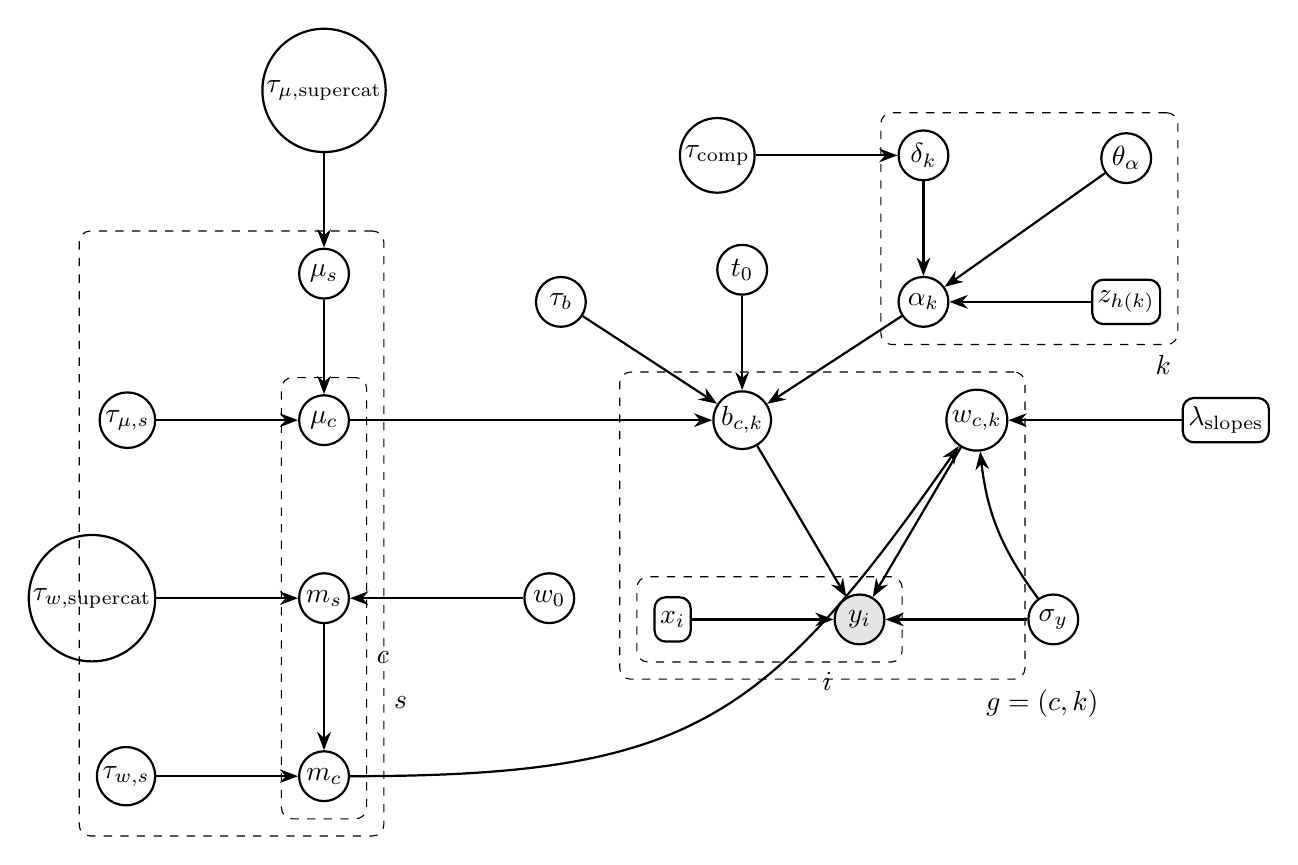
\begin{tikzpicture}
  % Species / supercategory hierarchy (intercepts + slope means).
  \node[rtlatent] (mu_s) {$\mu_s$};
  \node[rtlatent, below=12mm of mu_s] (mu_c) {$\mu_c$};
  \node[rtlatent, above=12mm of mu_s] (tau_mu_sc) {$\tau_{\mu,\mathrm{supercat}}$};
  \node[rtlatent, left=18mm of mu_c] (tau_mu_s) {$\tau_{\mu,s}$};

  \node[rtlatent, below=16mm of mu_c] (m_s) {$m_s$};
  \node[rtlatent, below=16mm of m_s] (m_c) {$m_c$};
  \node[rtlatent, left=18mm of m_s] (tau_w_sc) {$\tau_{w,\mathrm{supercat}}$};
  \node[rtlatent, left=18mm of m_c] (tau_w_s) {$\tau_{w,s}$};
  \node[rtlatent, right=22mm of m_s] (w0) {$w_0$};

  % Group-level coefficients (per (species, compound)).
  \node[rtlatent, right=46mm of mu_c] (b) {$b_{c,k}$};
  \node[rtlatent, right=22mm of b] (w) {$w_{c,k}$};
  \node[rtlatent, above=12mm of b] (t0) {$t_0$};
  \node[rtlatent, above left=10mm and 18mm of b] (tau_b) {$\tau_b$};
  \node[rtconst, right=22mm of w] (lambda) {$\lambda_{\mathrm{slopes}}$};

  % Chemistry-informed compound effects.
  \node[rtlatent, above right=10mm and 18mm of b] (alpha) {$\alpha_k$};
  \node[rtlatent, above=12mm of alpha] (delta) {$\delta_k$};
  \node[rtlatent, left=18mm of delta] (tau_comp) {$\tau_{\mathrm{comp}}$};
  \node[rtconst, right=18mm of alpha] (z) {$z_{h(k)}$};
  \node[rtlatent, above=12mm of z] (theta) {$\theta_\alpha$};

  % Observation model.
  \coordinate (bw_mid) at ($(b)!0.5!(w)$);
  \node[rtobs, below=22mm of bw_mid] (y) {$y_i$};
  \node[rtconst, left=18mm of y] (x) {$x_i$};
  \node[rtlatent, right=18mm of y] (sigma_y) {$\sigma_y$};

  % Edges.
  \path[rtarrow]
    (tau_mu_sc) edge (mu_s)
    (mu_s) edge (mu_c)
    (tau_mu_s) edge (mu_c)

    (w0) edge (m_s)
    (tau_w_sc) edge (m_s)
    (m_s) edge (m_c)
    (tau_w_s) edge (m_c)

    (t0) edge (b)
    (tau_b) edge (b)
    (mu_c) edge (b)
    (alpha) edge (b)

    (m_c) edge[out=0, in=235, looseness=1.25] (w)
    (lambda) edge (w)

    (x) edge (y)
    (b) edge (y)
    (w) edge (y)
    (sigma_y) edge (y)
    (sigma_y) edge[bend left=15] (w)

    (tau_comp) edge (delta)
    (delta) edge (alpha)
    (z) edge (alpha)
    (theta) edge (alpha);

  % Plates (drawn behind nodes).
  \begin{scope}[on background layer]
    \node[rtplate, fit=(mu_c) (m_c), label=below right:{$c$}] (plate_c) {};
    \node[rtplate, fit=(mu_s) (m_s) (tau_mu_s) (tau_w_s) (plate_c), label=below right:{$s$}] {};
    \node[rtplate, fit=(alpha) (delta) (z), label=below right:{$k$}] {};
    \node[rtplate, fit=(x) (y), label=below right:{$i$}] (plate_i) {};
    \node[rtplate, fit=(b) (w) (plate_i), label=below right:{$g=(c,k)$}] {};
  \end{scope}
\end{tikzpicture}
\caption{Plate diagram for the partial pooling RT ridge model. Shaded nodes are observed. Vector-valued nodes implicitly range over run covariates ($1\!:\!p$) or embedding dimensions ($1\!:\!D$). In production, the per-group slopes $w_{c,k}$ are integrated out (collapsed ridge) during inference and then recovered in closed form after fitting the hyperparameters.}
\label{fig:rt_partial_pool_plate}
\end{figure}

\paragraph{Interpretation.}
The intercept $b_{c,k}$ represents the baseline RT of compound $k$ in species $c$; we expect related species in the same
supercategory to have similar baselines, and we expect chemically similar compounds to have similar baselines, so we pool
both species and compound effects. The slope coefficients $w_{c,k,j}$ capture how run conditions shift RT; because run
covariates are correlated, we use ridge shrinkage for stability and we pool slope means at the species and supercategory
levels.

\subsection{Likelihood}

Conditioned on group-level coefficients:
\[
  p(\{y_i\}\mid \{b_{c,k}\}, \{w_{c,k,j}\}, \sigma^2)
  = \prod_{i} \mathcal{N}\!\left(
    y_i \mid b_{c(i),k(i)} + \sum_{j=1}^{p} x_{i,j}\,w_{c(i),k(i),j}, \sigma^2
  \right).
\]

\subsection{Priors (partial pooling + chemistry)}

\paragraph{What pooling means (and what ``partial pooling'' is).}
Pooling is how a model shares information across related groups when some groups have little data. In a regression with
many groups, there are three common extremes:
\begin{itemize}
  \item \textbf{No pooling:} fit each group completely independently (high variance in sparse groups).
  \item \textbf{Full pooling:} force groups to share the same parameter (low variance, but can underfit real
  between-group differences).
  \item \textbf{Partial pooling:} learn group-specific parameters while shrinking them toward a shared mean, with the
  amount of shrinkage learned from the data.
\end{itemize}
Hierarchical priors implement partial pooling: each group parameter is drawn from a distribution centered at a
population-level mean, and the population scales (e.g., $\tau_{\mu,\cdot}$ and $\tau_{w,\cdot}$ below) determine how
strongly groups are pulled together.

\paragraph{Where partial pooling happens in this model.}
Partial pooling occurs in two places. First, the intercept hierarchy pools baseline RTs across \texttt{species} within a
\texttt{species\_cluster} (supercategory / matrix) (via $\mu_c \leftarrow \mu_{s(c)}$), stabilizing rare species. Second,
the slope-mean hierarchy pools the run-effect means $m_{c,j}$ across \texttt{species} within each \texttt{species\_cluster},
improving stability of run-covariate effects under correlated predictors. Separately, the compound prior pools across
compounds through a chemistry-informed mean (ChemBERTa embeddings), which is especially helpful when a compound has
limited history.

\paragraph{Intercepts: species + compound baseline with partial pooling.}
We shrink each group intercept toward an additive species and compound baseline:
\[
  b_{c,k} \sim \mathcal{N}\!\left(t_0 + \mu_c + \alpha_k,\; \tau_b^2\right).
\]
In this prior, $t_0$ denotes a global intercept shared across all groups, $\mu_c$ is a species-specific intercept offset,
$\alpha_k$ is a compound baseline shared across species, and $\tau_b$ controls residual group-level variation around the
hierarchical mean.

Species offsets are pooled within supercategory:
\[
  \mu_s \sim \mathcal{N}(0,\tau_{\mu,\mathrm{supercat}}^2), \qquad
  \mu_c \sim \mathcal{N}\!\left(\mu_{s(c)}, \tau_{\mu,s(c)}^2\right).
\]
The mapping $s(c)$ assigns each species $c$ to its enclosing \texttt{species\_cluster} $s$. $\mu_s$ is a supercategory-level
offset, and $\tau_{\mu,\mathrm{supercat}}$ and $\tau_{\mu,s}$ control pooling strength at the supercategory and
within-supercategory levels, respectively.
We allow supercategory-specific pooling strength by learning $\tau_{\mu,s}$ per supercategory (with a shared prior).

\paragraph{Compound effects: chemistry-informed prior mean.}
We model the compound effect as a chemistry-driven mean plus a residual:
\[
  z_{h,d} = e_{h,d} - \bar{e}_{d,\text{train}}, \qquad
  \alpha_k = \sum_{d=1}^{D} z_{h(k),d}\,\theta_{\alpha,d} + \delta_k,
\]
\[
  \theta_{\alpha,d} \sim \mathcal{N}(0, \sigma_\theta^2)\quad(d=1,\ldots,D), \qquad
  \delta_k \sim \mathcal{N}(0,\tau_{\mathrm{comp}}^2).
\]
Let $e_{h,d}$ be the fixed ChemBERTa embedding for chemical identifier $h$ and dimension $d$, and let $\bar{e}_{d,\text{train}}$
be the training mean for dimension $d$; then $z_{h,d}$ is the centered embedding. The weights $\theta_{\alpha,d}$ map
embeddings to a prior mean for the compound baseline $\alpha_k$ (with prior scale $\sigma_\theta$), while $\delta_k$ is a
compound-specific residual with scale $\tau_{\mathrm{comp}}$.
Centering $z_{h,d}$ by the training mean $\bar{e}_{d,\text{train}}$ and enforcing mean-zero constraints on compound
offsets are convenient reparameterizations for identifiability with $t_0$.

\paragraph{Slopes on run covariates: ridge with hierarchical slope means.}
We use a ridge prior on per-group slopes around a species-level slope mean. For each run covariate $j=1,\ldots,p$:
\[
  w_{c,k,j} \sim \mathcal{N}\!\left(m_{c,j},\; \sigma^2/\lambda_{\mathrm{slopes}}\right),
\]
where $w_{c,k,j}$ is the slope for group $(c,k)$ on covariate $j$, $m_{c,j}$ is a species-level slope mean, $\sigma^2$ is
the residual variance from the likelihood, and $\lambda_{\mathrm{slopes}}$ is a fixed ridge penalty (precision) that
controls shrinkage toward $m_{c,j}$. We pool $m_{c,j}$ through the supercategory:
\[
  w_{0,j} \sim \mathcal{N}(0, \sigma_{w0}^2), \qquad
  m_{s,j} \sim \mathcal{N}(w_{0,j},\tau_{w,\mathrm{supercat}}^2), \qquad
  m_{c,j} \sim \mathcal{N}(m_{s(c),j},\tau_{w,s(c)}^2).
\]
In this hierarchy, $w_{0,j}$ is a global slope mean for covariate $j$ (with prior scale $\sigma_{w0}$), $m_{s,j}$ is a
supercategory-level slope mean, and $\tau_{w,\mathrm{supercat}}$ and $\tau_{w,s}$ control pooling strength across
supercategories and within each supercategory.
As with the intercept hierarchy, we allow supercategory-specific pooling strength by learning $\tau_{w,s}$ per
supercategory (with a shared prior).

\paragraph{What ``ridge'' means (and why not lasso).}
A ridge prior is a Gaussian prior on coefficients. In a linear model, this corresponds to an $\ell_2$ shrinkage penalty:
large coefficients are discouraged, but coefficients are not driven exactly to zero.
This behavior is a good fit for run covariates that are highly correlated (common for \texttt{IS*}/\texttt{ES\_\*}):
ridge shrinkage distributes weight smoothly across correlated predictors and yields more stable fits.
By contrast, lasso corresponds to a Laplace prior ($\ell_1$ penalty) and tends to select an arbitrary subset of
correlated covariates, producing unstable coefficients across retrains and brittle behavior in sparse groups.

\paragraph{Noise and scale priors.}
We model residual noise with:
\[
  \sigma_y \sim \mathrm{HalfNormal}(\sigma_{y,\mathrm{prior}}), \qquad \sigma^2 = \sigma_y^2,
\]
and use HalfNormal priors for positive scales such as $\tau_b$, $\tau_{\mu,\mathrm{supercat}}$, $\tau_{\mu,s}$,
$\tau_{w,\mathrm{supercat}}$, $\tau_{w,s}$, and $\tau_{\mathrm{comp}}$.

\subsection{Inference and predictive uncertainty}

We fit the model with variational inference (ADVI), which approximates the posterior over the hierarchical parameters
with a tractable distribution (rather than running full MCMC). This makes training feasible at production scale.

\paragraph{Collapsed slopes (why it is fast).}
The dominant parameter count in a fully explicit model would be the per-group slope coefficients $w_{c,k,1:p}$
(one set per \texttt{(species, comp\_id)} pair). Instead of representing all of these slopes as latent nodes in the PyMC
graph, we \textbf{collapse} them: conditional on the ridge prior and the run covariates, the slopes can be integrated out
analytically. In practice we precompute small per-group sufficient statistics, such as
$S^{xx}_{g,j\ell}=\sum_{i:g(i)=g} x_{i,j}x_{i,\ell}$ and $S^{xy}_{g,j}=\sum_{i:g(i)=g} x_{i,j}y_i$, and use the resulting
collapsed (marginal) likelihood inside ADVI. This replaces a very large set of per-row computations with compact per-group
summaries, which is the main speedup.
Appendix~\ref{app:collapsed_slopes} derives the collapsed likelihood and the corresponding closed-form posterior for
$w_{g,1:p}$.
We still represent per-group intercepts $b_{c,k}$ explicitly because they are tied to the hierarchical prior mean
$t_0+\mu_c+\alpha_k$.

\paragraph{Stage-1 coefficient summaries.}
After ADVI fits global and hierarchical parameters (including the intercept hierarchy and the slope-mean hierarchy), we
recover a Gaussian posterior for each group’s coefficients in closed form and export per-group summaries for
$\beta_{c,k,0}=b_{c,k}$ and $\beta_{c,k,j}=w_{c,k,j}$ for $j=1,\ldots,p$ (posterior mean and covariance). This exported
artifact is what we use in production scoring: it avoids running Bayesian inference at runtime while still providing an
explicit uncertainty estimate for RT filtering.

\textbf{Approximation note:} we compute these group-wise posteriors conditional on fitted hyperparameters (typically at
their posterior means under ADVI), rather than fully integrating over hyperparameter uncertainty.

The group-wise coefficient posterior depends on global and hierarchical parameters such as $t_0$, the pooling scales
($\tau_{\mu,\cdot}$, $\tau_{w,\cdot}$, $\tau_{\mathrm{comp}}$), chemistry weights $\theta_{\alpha,1},\ldots,\theta_{\alpha,D}$,
and the noise scale $\sigma_y$. A fully Bayesian prediction would average over uncertainty in these quantities; we instead
``plug in'' their fitted values and compute the conditional Gaussian posterior for each group in closed form. This is a
plug-in (point-estimate) approximation (sometimes called empirical Bayes): it makes scoring simple and deterministic,
but it can slightly understate uncertainty if hyperparameters are themselves uncertain.

At scoring time, for a new row $i$ we select the coefficient-summary group $g(i)$, use posterior mean coefficients for a
point prediction, and propagate coefficient uncertainty into a predictive variance:
\[
  \hat{y}_i = b_{g(i)} + \sum_{j=1}^{p} x_{i,j}\,w_{g(i),j}, \qquad
  \widehat{\mathrm{Var}}(y_i\mid x_{i,1:p}) \approx \sigma^2_{g(i)} + \sum_{a=0}^{p}\sum_{b=0}^{p}
  \tilde{x}_{i,a}\tilde{x}_{i,b}\,\widehat{\mathrm{Cov}}(\beta_{g(i),a},\beta_{g(i),b}),
\]
where $\tilde{x}_{i,0}=1$ and $\tilde{x}_{i,j}=x_{i,j}$ for $j=1,\ldots,p$.
In the hierarchical ridge model $\sigma^2_{g}$ is shared across groups, while the sklearn supercategory ridge baseline
estimates a separate $\sigma^2_{g}$ per \texttt{(species\_cluster, comp\_id)} pair.
With $\hat{\sigma}_i=\sqrt{\widehat{\mathrm{Var}}(y_i\mid x_{i,1:p})}$, a nominal 95\% RT window is
$\hat{y}_i \pm k_{0.95}\,\hat{\sigma}_i$ (width $2\cdot k_{0.95}\cdot \hat{\sigma}_i$), where
$k_{0.95}=\Phi^{-1}(0.975)\approx 1.96$ under a Normal approximation. This window can vary by group and by
covariates because it includes both residual noise and coefficient uncertainty.
Downstream peak assignment uses this interval as a filter: a candidate peak is retained when its observed RT falls within
the model’s window around $\hat{y}_i$.

For contrast, the production lasso baseline attaches a fixed window estimated from a worksheet-level hold-out split
(described in the lasso baseline section below).

\section{Evaluation}

We compare models trained on the cap100 dataset (capped at 100 observations per (species, comp\_id) pair) and
evaluated on realtest for lib208 and lib209. This report focuses on
\textbf{seen-compound performance}: the standard realtest evaluation where models score nearly all rows and the
comparison is driven by accuracy and calibrated windows rather than missing-model fallbacks.
To focus on \emph{model form} rather than feature engineering, we use the same linear run covariates for all models
(no polynomial expansions).

\paragraph{Metrics.}
Let $y_i$ be observed RT and $\hat{y}_i$ the point prediction (minutes).
\begin{itemize}
  \item \textbf{RMSE}: $\sqrt{\frac{1}{n}\sum_i (\hat{y}_i - y_i)^2}$.
  \item \textbf{MAE}: $\frac{1}{n}\sum_i |\hat{y}_i - y_i|$.
  \item \textbf{Cov95} (ridge models): define predicted variance as
  \[
  \begin{aligned}
    \widehat{\mathrm{Var}}(y_i\mid x_{i,1:p})
    &\approx \sigma^2_{g(i)} \\
    &\quad + \sum_{a=0}^{p}\sum_{b=0}^{p}
      \tilde{x}_{i,a}\tilde{x}_{i,b}\,
      \widehat{\mathrm{Cov}}\!\left(\beta_{g(i),a},\beta_{g(i),b}\right),
  \end{aligned}
  \]
  with predicted standard deviation $\hat{\sigma}_i=\sqrt{\widehat{\mathrm{Var}}(y_i\mid x_{i,1:p})}$ and
  $k_{0.95}=\Phi^{-1}(0.975)\approx 1.96$.
  We define the nominal 95\% interval as $\hat{y}_i \pm k_{0.95}\,\hat{\sigma}_i$ and count row $i$ as ``covered'' if
  $|\hat{y}_i - y_i| \le k_{0.95}\,\hat{\sigma}_i$; Cov95 is the empirical fraction of covered rows.
  The terms $\sigma^2_{g(i)}$ and $\widehat{\mathrm{Cov}}(\beta_{g(i)})$ come from the exported stage-1 coefficient summaries:
  for the sklearn ridge baseline they are computed analytically from ridge normal equations with an inverse-gamma noise prior,
  while for the partial pooling model they are computed in closed form conditional on fitted hierarchical hyperparameters
  (an empirical-Bayes plug-in approximation).
  \item \textbf{Width95} (ridge models): $\frac{1}{n}\sum_i 2\cdot k_{0.95}\cdot \hat{\sigma}_i$.
\end{itemize}

In the expressions above, $g(i)$ denotes the coefficient-summary group for row $i$, and we use the augmented covariates
$\tilde{x}_{i,0}=1$ and $\tilde{x}_{i,j}=x_{i,j}$ for $j=1,\ldots,p$.
For the production lasso baseline, the ``window'' is a fixed filtering half-width derived from held-out residuals and then
scaled by a global multiplier (see lasso baseline section below). This window is not calibrated to a nominal 95\% target,
so we do not report it as Cov95/Width95.

\subsection{Alternative model: supercategory ridge (sklearn)}

As a fast baseline, we fit an independent ridge regression for each group
$(\texttt{species\_cluster},\texttt{comp\_id})$ using the same run covariates. This model has no hierarchy across
\texttt{species} and no chemistry: each supercategory--compound pair is fit essentially independently, with an $\ell_2$
penalty for stability under correlated covariates.
We attach an approximate Normal predictive distribution by combining an estimated noise scale with an approximate
coefficient covariance.

\paragraph{Windowing.}
For each \texttt{(species\_cluster, comp\_id)} group this baseline stores a fitted coefficient mean, an approximate
coefficient covariance, and an estimated residual variance $\sigma^2_g$. For a new row, we compute $\hat{y}_i$ and
$\hat{\sigma}_i$ and use the nominal 95\% window $\hat{y}_i \pm k_{0.95}\,\hat{\sigma}_i$ (as defined above). This yields a
row-specific window rather than a fixed width per model.

\begin{figure}[H]
\centering
\small
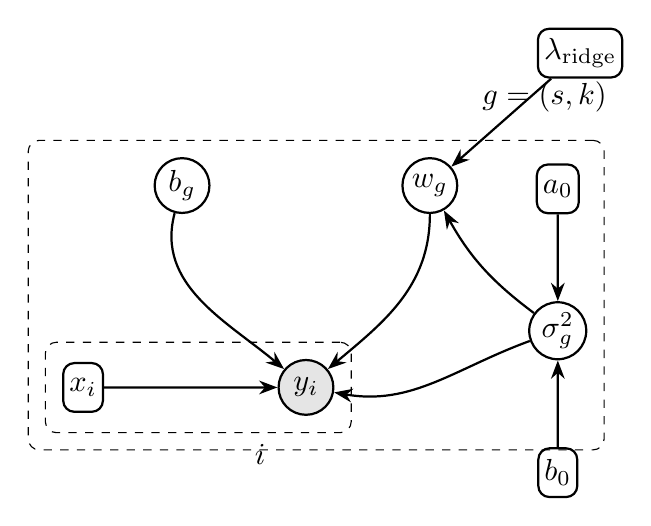
\begin{tikzpicture}[scale=1.1, transform shape]
  % Group-level parameters (independent per group).
  \node[rtlatent] (b) {$b_g$};
  \node[rtlatent, right=22mm of b] (w) {$w_g$};
  \node[rtlatent, below right=12mm and 10mm of w] (sig2) {$\sigma_g^2$};
  \node[rtconst, above right=10mm and 10mm of w] (lambda) {$\lambda_{\mathrm{ridge}}$};
  \node[rtconst, above=10mm of sig2] (a0) {$a_0$};
  \node[rtconst, below=10mm of sig2] (b0) {$b_0$};

  % Observations.
  \coordinate (bw_mid) at ($(b)!0.5!(w)$);
  \node[rtobs, below=20mm of bw_mid] (y) {$y_i$};
  \node[rtconst, left=20mm of y] (x) {$x_i$};

  % Edges (interpret ridge as a Gaussian prior / penalty on slopes).
  \path[rtarrow]
    (a0) edge (sig2)
    (b0) edge (sig2)
    (lambda) edge (w)
    (sig2) edge[bend left=12] (w)
    (b) edge[out=255, in=140] (y)
    (w) edge[out=270, in=40] (y)
    (sig2) edge[out=200, in=-10] (y)
    (x) edge (y);

  % Plates.
  \begin{scope}[on background layer]
    \node[rtplate, fit=(x) (y), label=below right:{$i$}] (plate_i) {};
    \node[rtplate, fit=(b) (w) (sig2) (plate_i), label={[yshift=2mm]above right:{$g=(s,k)$}}] {};
  \end{scope}
\end{tikzpicture}
\caption{Plate diagram for the sklearn supercategory ridge baseline. Each group $g=(s,k)$ (species\_cluster, comp\_id) is fit independently with ridge shrinkage on slopes $w_g$ (intercept $b_g$ unpenalized). The exported artifact stores a coefficient mean, an approximate coefficient covariance, and a per-group residual variance estimate $\sigma_g^2$ (from an inverse-gamma noise model with hyperparameters $a_0,b_0$).}
\label{fig:rt_sklearn_ridge_plate}
\end{figure}

\subsection{Baseline currently in production: supercategory lasso}

The production baseline is a bank of lasso regressions fit per \texttt{(species\_cluster, comp\_id)} pair. Lasso is
attractive for sparse solutions, but its $\ell_1$ prior is a poor match to correlated run covariates and it does not
support partial pooling or chemistry-informed sharing across compounds. Its ``interval'' is a fixed window, not a
probabilistic prediction interval.

\paragraph{Windowing in Hippopotamus.}
In Hippopotamus, lasso coefficients are fit on a worksheet-level train split, and then a fixed window is attached using a
hold-out split (commonly an 80/20 split by worksheet). For each \texttt{(species\_cluster, comp\_id)} model, the stored
\texttt{window} is computed from the held-out residuals as a high percentile of the absolute error (approximately
``$6\sigma$'' under a Normal error model):
\[
  w_{\mathrm{base}} = \mathrm{quantile}_{q}(|\hat{y}-y|),\qquad q\approx 0.999999998,
\]
and is saved alongside the regression coefficients in the model bundle. At scoring time (Sally/Hippopotamus), the
effective filter half-width is scaled by a global multiplier and clamped to a minimum:
\[
  w_i = m\cdot \max(w_{\mathrm{base}}, w_{\min}),
\]
with default $m=4$ and $w_{\min}=0.001$. Candidate peaks are retained when $|\hat{y}_i - y_i| \le w_i$.
This is a pragmatic way to set windows, but it is not derived from an explicit predictive distribution and it does not
provide row-specific uncertainty; the window depends on the chosen split and this heuristic scale rule.

\begin{figure}[H]
\centering
\small
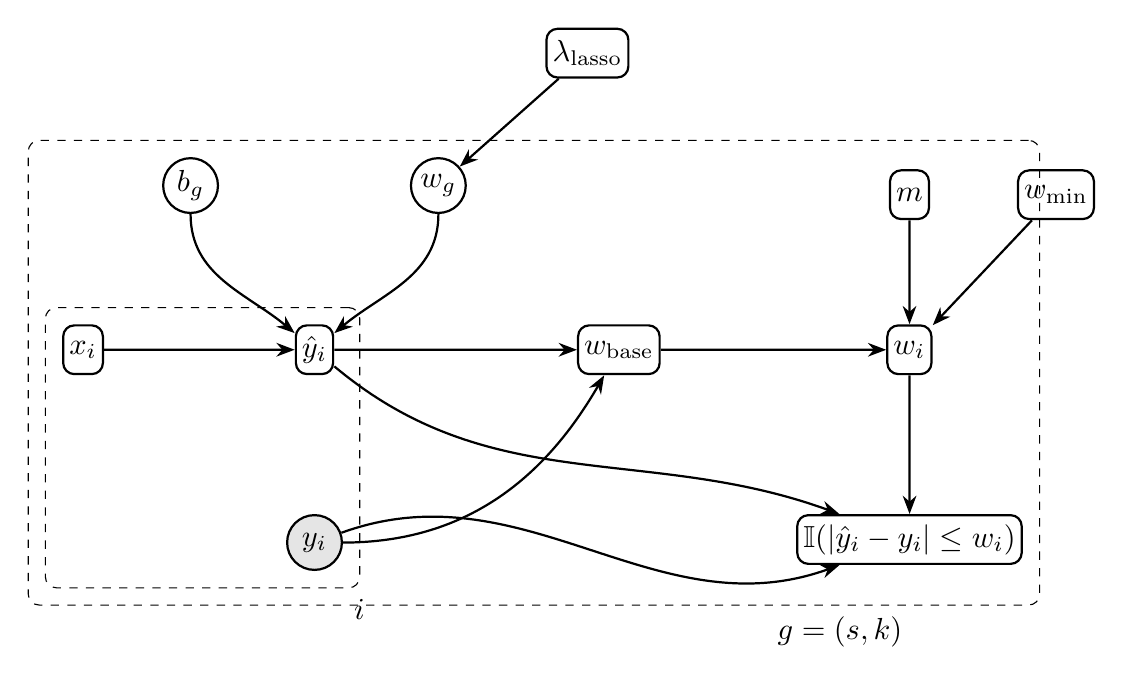
\begin{tikzpicture}[scale=1.1, transform shape]
  % Lasso point-estimate coefficients (independent per group).
  \node[rtlatent] (b) {$b_g$};
  \node[rtlatent, right=22mm of b] (w) {$w_g$};
  \node[rtconst, above right=10mm and 10mm of w] (alpha) {$\lambda_{\mathrm{lasso}}$};

  % Prediction + window heuristic.
  \coordinate (bw_mid) at ($(b)!0.5!(w)$);
  \node[rtconst, below=16mm of bw_mid] (yhat) {$\hat{y}_i$};
  \node[rtconst, left=22mm of yhat] (x) {$x_i$};
  \node[rtobs, below=16mm of yhat] (y) {$y_i$};

  \node[rtconst, right=28mm of yhat] (wbase) {$w_{\mathrm{base}}$};
  \node[rtconst, right=26mm of wbase] (wi) {$w_i$};
  \node[rtconst, below=16mm of wi] (keep) {$\mathbb{I}(|\hat{y}_i-y_i|\le w_i)$};

  \node[rtconst, above=12mm of wi] (m) {$m$};
  \node[rtconst, right=10mm of m] (wmin) {$w_{\min}$};

  % Edges.
  \path[rtarrow]
    (alpha) edge (w)
    (b) edge[out=270, in=140] (yhat)
    (w) edge[out=270, in=40] (yhat)
    (x) edge (yhat)
    (yhat) edge[out=0, in=180] (wbase)
    (y) edge[out=0, in=240] (wbase)
    (wbase) edge (wi)
    (m) edge (wi)
    (wmin) edge (wi)
    (wi) edge (keep)
    (yhat) edge[out=320, in=160] (keep)
    (y) edge[out=20, in=200] (keep);

  % Plates.
  \begin{scope}[on background layer]
    \node[rtplate, fit=(x) (yhat) (y), label=below right:{$i$}] (plate_i) {};
    \node[rtplate, fit=(b) (w) (plate_i) (wbase) (wi) (keep), label=below right:{$g=(s,k)$}] {};
  \end{scope}
\end{tikzpicture}
\caption{Plate diagram for the production supercategory lasso baseline (Hippopotamus). For each group $g=(s,k)$ (species\_cluster, comp\_id), lasso fits point-estimate coefficients $(b_g,w_g)$ and computes a fixed window $w_{\mathrm{base}}$ from held-out absolute errors; scoring scales and clamps it to $w_i=m\max(w_{\mathrm{base}},w_{\min})$ and keeps a candidate when $|\hat{y}_i-y_i|\le w_i$.}
\label{fig:rt_lasso_plate}
\end{figure}

\section{Results (seen compounds)}

\subsection{Global performance}

Table~\ref{tab:global_metrics} summarizes global metrics on realtest for lib208 and lib209. Lasso baselines do not
score all rows; \textbf{Rows scored} reflects applicability.

\begin{table}[H]
\centering
\caption{Global realtest metrics for cap100-trained models (linear features). Cov95/Width95 report empirical coverage and
mean width of the nominal 95\% Normal interval $\hat{y}_i \pm k_{0.95}\,\hat{\sigma}_i$ and are only defined for ridge
models with an explicit predictive variance. The lasso baseline uses a heuristic fixed filtering window; its Cov95/Width95
entries are omitted (--) to avoid implying nominal calibration.}
\label{tab:global_metrics}
\begin{tabular}{llrrrrrr}
\toprule
Lib & Model & RMSE & MAE & Cov95 & Width95 & Rows scored & Train (min) \\
\midrule
208 & Ridge (supercategory) & 0.009050 & 0.004684 & 0.944 & \textbf{0.023573} & \textbf{100.0\%} & \textbf{0.0} \\
208 & Ridge (partial pooling) & \textbf{0.007846} & \textbf{0.003817} & \textbf{0.958} & 0.028744 & \textbf{100.0\%} & 129.8 \\
208 & Lasso (supercategory) & 0.015081 & 0.007956 & -- & -- & 94.7\% & -- \\
\midrule
209 & Ridge (supercategory) & 0.008295 & 0.004631 & 0.919 & \textbf{0.020994} & \textbf{100.0\%} & \textbf{0.0} \\
209 & Ridge (partial pooling) & \textbf{0.007589} & \textbf{0.004203} & \textbf{0.957} & 0.027094 & \textbf{100.0\%} & 230.6 \\
209 & Lasso (supercategory) & 0.009439 & 0.004954 & -- & -- & 97.8\% & -- \\
\bottomrule
\end{tabular}
\end{table}

\paragraph{Interpretation.}
Relative to Ridge (supercategory), Ridge (partial pooling) improves RMSE while moving coverage
closer to the nominal 0.95 target. This is desirable for peak assignment because under-coverage translates directly into
missed true peaks when the window is used as a hard filter.
The lasso baseline is included for context: it does not score all rows and its uncertainty is a fixed window rather than
a probabilistic interval.

\begin{figure}[H]
\centering
\includegraphics[width=0.95\linewidth]{lib208_global_comparison_anchor_none_full.png}
\caption{Global comparison across report baselines for lib208 (cap100 training, realtest evaluation). Panels show RMSE,
Cov95 (ridge models only; lasso omitted), and mean RT window width (Width95 for ridge models; production filtering window
for lasso). Tighter windows are only meaningful when coverage is comparable.}
\label{fig:global_comparison_lib208}
\end{figure}

\begin{figure}[H]
\centering
\includegraphics[width=0.95\linewidth]{lib209_global_comparison_anchor_none_full.png}
\caption{Global comparison across report baselines for lib209 (cap100 training, realtest evaluation). Panels show RMSE,
Cov95 (ridge models only; lasso omitted), and mean RT window width (Width95 for ridge models; production filtering window
for lasso). Tighter windows are only meaningful when coverage is comparable.}
\label{fig:global_comparison_lib209}
\end{figure}

\subsection{Interval calibration: supercategory ridge vs partial pooling}

The sklearn ridge baseline and the proposed hierarchical ridge model are both linear in the same run covariates, but
they differ in how information is shared across sparse groups and in how predictive variance is formed. Empirically, the
sklearn baseline produces narrower windows but under-covers the nominal 95\% target (coverage $\sim$0.92--0.94). The
hierarchical model yields coverage closer to nominal at moderately larger width.

\subsection{Performance by species\_cluster}

Figures~\ref{fig:by_cluster_lib208} and \ref{fig:by_cluster_lib209} aggregate metrics by \texttt{species\_cluster}.

\begin{figure}[H]
\centering
\includegraphics[width=0.95\linewidth]{lib208_by_species_cluster_anchor_none_full.png}
\caption{Metrics by \texttt{species\_cluster} (supercategory) for lib208 report baselines. The Cov95 panel excludes lasso
because its fixed filtering window is not a nominal probabilistic interval; mean RT window width includes the lasso
filtering window for context.}
\label{fig:by_cluster_lib208}
\end{figure}

\begin{figure}[H]
\centering
\includegraphics[width=0.95\linewidth]{lib209_by_species_cluster_anchor_none_full.png}
\caption{Metrics by \texttt{species\_cluster} (supercategory) for lib209 report baselines. The Cov95 panel excludes lasso
because its fixed filtering window is not a nominal probabilistic interval; mean RT window width includes the lasso
filtering window for context.}
\label{fig:by_cluster_lib209}
\end{figure}

\section{Preliminary end-to-end Sally evaluation (real sample sets)}

Offline split evaluation is necessary but not sufficient for deployment: in production the RT model is used inside
Sally's peak assignment pipeline as a hard filter and interacts with other stages (candidate generation, peak selection,
and post-processing). To assess the impact in context, we ran Sally end-to-end on real sample sets using
\texttt{sally-dev evaluate} and compared:
\begin{itemize}
  \item the current production baseline RT model (\textbf{supercategory lasso}, model type \texttt{ESLASSO}), and
  \item the new CompAssign partial pooling ridge model exported as stage-1 coefficient summaries
  (model type \nolinkurl{COMPASSIGN_PP_RIDGE}).
\end{itemize}

All evaluations use the \texttt{mdsutils} metric implementation (precision/recall/Threat Score) to match current Sally
reporting, and were run with the standard \texttt{baseline} peak-assignment method.
To make iteration practical, we relied on Sally's local on-disk cache to avoid expensive peak fetches on repeated runs.

\paragraph{What changed in Sally (summary).}\mbox{}\\
To support \nolinkurl{COMPASSIGN_PP_RIDGE} end-to-end inside \texttt{sally-dev}, we made the following focused changes:
\begin{itemize}
  \item \textbf{New modelType.} Added \nolinkurl{modelType=COMPASSIGN_PP_RIDGE} which loads CompAssign stage-1 coefficient
  summaries and backoff summaries (both shipped as \texttt{.npz} artifacts), and computes per-task RT windows from
  predictive variance.
  \item \textbf{RT window plumbing.} Generalized \texttt{RegressionPredictor} so RT windows can be either per-compound
  (1D) or per-(task,compound) (2D), since \nolinkurl{COMPASSIGN_PP_RIDGE} produces row-specific uncertainty.
  \item \textbf{sally-dev flag pass-through.} Added CompAssign RT inputs (species, species\_cluster, and covariates CSV) and
  \texttt{--force-curate} to run the full curation pipeline for evaluation even when a sample set would normally be
  skipped.
  \item \textbf{Evaluation reliability and covariates I/O.} Updated \texttt{sally-dev evaluate} to fail fast when the
  underlying pipeline run fails (instead of continuing with stale cached pickles), and updated the pipeline wrapper and
  \nolinkurl{COMPASSIGN_PP_RIDGE} loader so production-style RT covariates can be mounted into the Docker container and read
  efficiently by streaming only the required task IDs (important for multi-GB lib209 covariates CSVs).
\end{itemize}

\paragraph{Selected SSIDs.}
We evaluated five held-out cell-type SSIDs from supercategories 6 and 8. For lib208:
\textbf{SSID 12307} (supercat 6), \textbf{SSID 12609} (supercat 8), and \textbf{SSID 12725} (supercat 6). For lib209:
\textbf{SSID 23059} (supercat 6) and \textbf{SSID 20159} (supercat 8).
For convenience and full reproducibility, \nolinkurl{src/compassign/rt/sally_test.sh} re-runs the exact SSIDs via
\texttt{sally-dev evaluate} (script: \path{external_repos/sally/scripts/sally-dev}).
We compare baseline \texttt{ESLASSO} vs candidate \nolinkurl{COMPASSIGN_PP_RIDGE} and write outputs into fixed
subdirectories under \path{external_repos/sally/out/}.
The script includes the exact parameters used (including covariates CSV paths) and prints a compact summary table.
These results require the Sally checkout under \nolinkurl{external_repos/sally} to be on branch
\nolinkurl{jw/new-experimental-model}.

\paragraph{Results.}
Tables~\ref{tab:sally_prelim_cells_lib208} and \ref{tab:sally_prelim_cells_lib209} report the end-to-end peak-assignment
metrics from Sally's \texttt{mdsutils} summary pickles. Higher is better for all three metrics. For each SSID, the
baseline and \nolinkurl{COMPASSIGN_PP_RIDGE} were run with the same peak-assignment method and evaluation mode.

\begin{table}[H]
\centering
\caption{Preliminary end-to-end Sally evaluation on selected cell-type SSIDs (lib208; supercategories 6 and 8). Metrics
are precision, recall, and Threat Score (TS) from \texttt{mdsutils}. Bold indicates the best value within each SSID.}
\label{tab:sally_prelim_cells_lib208}
\begin{tabular}{lllrrr}
\toprule
Supercat & SSID & Model & Precision & Recall & TS \\
\midrule
6 & 12307 & ESLASSO (supercategory lasso) & 0.8436 & 0.7848 & 0.6851 \\
6 & 12307 & COMPASSIGN\_PP\_RIDGE (partial pooling ridge) & \textbf{0.9537} & \textbf{0.8109} & \textbf{0.7801} \\
\midrule
8 & 12609 & ESLASSO (supercategory lasso) & 0.8553 & 0.6513 & 0.5867 \\
8 & 12609 & COMPASSIGN\_PP\_RIDGE (partial pooling ridge) & \textbf{0.8591} & \textbf{0.8036} & \textbf{0.7101} \\
\midrule
6 & 12725 & ESLASSO (supercategory lasso) & 0.6808 & 0.8610 & 0.6134 \\
6 & 12725 & COMPASSIGN\_PP\_RIDGE (partial pooling ridge) & \textbf{0.8587} & \textbf{0.8786} & \textbf{0.7676} \\
\bottomrule
\end{tabular}
\end{table}

\begin{table}[H]
\centering
\caption{Preliminary end-to-end Sally evaluation on selected cell-type SSIDs (lib209; supercategories 6 and 8). Metrics
are precision, recall, and Threat Score (TS) from \texttt{mdsutils}. Bold indicates the best value within each SSID.}
\label{tab:sally_prelim_cells_lib209}
\begin{tabular}{lllrrr}
\toprule
Supercat & SSID & Model & Precision & Recall & TS \\
\midrule
8 & 20159 & ESLASSO (supercategory lasso) & 0.8865 & 0.8697 & 0.7825 \\
8 & 20159 & COMPASSIGN\_PP\_RIDGE (partial pooling ridge) & \textbf{0.8967} & \textbf{0.8841} & \textbf{0.8024} \\
\midrule
6 & 23059 & ESLASSO (supercategory lasso) & 0.8357 & 0.5940 & 0.5319 \\
6 & 23059 & COMPASSIGN\_PP\_RIDGE (partial pooling ridge) & \textbf{0.8383} & \textbf{0.6667} & \textbf{0.5907} \\
\bottomrule
\end{tabular}
\end{table}

\paragraph{Provenance.}\mbox{}\\
Tables~\ref{tab:sally_prelim_cells_lib208} and \ref{tab:sally_prelim_cells_lib209} were computed from the \texttt{mdsutils}
summary pickles produced by \texttt{sally-dev evaluate} (script: \path{external_repos/sally/scripts/sally-dev}).
The exact output directories and summary pickle paths are recorded under \path{external_repos/sally/out/} and are
referenced/printed by \nolinkurl{src/compassign/rt/sally_test.sh}.

\paragraph{Interpretation (current status).}\mbox{}\\
Across these selected SSIDs, \nolinkurl{COMPASSIGN_PP_RIDGE} improves Threat Score (TS) relative to the current lasso
baseline on all three lib208 checks and both lib209 checks. These results are preliminary but are directionally
consistent with the offline split evaluations for lib208: partial pooling with a ridge prior can stabilize RT filtering
in hard cell-type supercategories.

\paragraph{Findings so far.}
On these selected cell-type SSIDs, \nolinkurl{COMPASSIGN_PP_RIDGE} improves TS by approximately +0.10 (SSID 12307),
+0.12 (SSID 12609), and +0.15 (SSID 12725) versus \texttt{ESLASSO} for lib208.
For lib209, \nolinkurl{COMPASSIGN_PP_RIDGE} improves TS by approximately +0.02 (SSID 20159) and +0.06 (SSID 23059).
Overall, the integration appears to be working end-to-end on both libraries and requires broader sampling to assess the
typical magnitude of gains.

\paragraph{Missing SMILES coverage.}
For these cap100-trained lib208/lib209 models, the coefficient-summary artifacts include compounds with missing chemistry
metadata (missing \texttt{chemical\_id} or missing ChemBERTa embeddings). For lib208, the trainer uses mean-embedding
fallback for 310 compounds with missing \texttt{chemical\_id} and 138 compounds with missing embeddings; for lib209, this is
990 and 540 compounds, respectively. This prevents coverage holes in the Sally integration (avoids ``No RT model'') at the
cost of disabling the chemistry-informed prior mean for those compounds (chemistry term uses $z_c=0$).

\paragraph{Recommended next steps.}
Before making a deployment decision, we recommend:
\begin{itemize}
  \item \textbf{Scale out evaluation.} Run the same baseline-vs-candidate comparison on a larger set of SSIDs (including
  multi-lib sample sets), reporting both per-SSID and aggregated deltas.
  \item \textbf{Remove manual inputs.} Implement automatic resolution of \texttt{species} and \texttt{species\_cluster}
  for each SSID (per lib) so \texttt{sally-dev evaluate} can be run reproducibly without hand-provided IDs.
  \item \textbf{Confirm end-to-end calibration.} Verify predictive window calibration (and its interaction with artifact
  and sparsity post-processing) across a broader sample of SSIDs.
\end{itemize}

\section{Discussion}

The offline split results establish that \texttt{COMPASSIGN\_PP\_RIDGE} improves RT prediction and produces calibrated
windows, but deployment impact depends on how RT filtering interacts with Sally's full peak-assignment pipeline. On five
real held-out SSIDs (Tables~\ref{tab:sally_prelim_cells_lib208} and \ref{tab:sally_prelim_cells_lib209}),
\nolinkurl{COMPASSIGN_PP_RIDGE} improves Threat Score (TS) versus the current \texttt{ESLASSO} baseline on all checks (lib208:
approximately +0.10, +0.12, +0.15; lib209: approximately +0.02, +0.06). This indicates the RT gains translate into
end-to-end improvements once post-processing (notably artifact handling) is aligned with the new RT filtering behavior.

Across both libraries, the hierarchical ridge model improves point accuracy modestly but, more importantly for peak
assignment, produces predictive windows with coverage close to the nominal 95\% target. The fast sklearn ridge baseline
is competitive in RMSE but systematically under-covers because its predictive variance is optimistic for many
supercategory--compound pairs. In a pipeline that uses RT windows as a hard filter, this under-coverage is not a cosmetic
issue: it directly increases the probability that the true peak is excluded from consideration.

The hierarchical model is designed around the data realities of RT regression. Species--compound history is sparse and
heavy-tailed, so independent per-group fits are unstable in the tail. Partial pooling addresses this by shrinking group
intercepts and slope means toward supercategory-aware priors, improving stability without sacrificing head performance.
Chemistry enters as a prior mean for compound effects, which lets the model share information across chemically similar
compounds and stabilizes estimates when per-compound support is limited.

The main practical downside is training cost: variational inference over the hierarchy is far slower than independent
ridge fits. This makes the hierarchical model best suited to offline retrains (periodic model refreshes), while the fast
sklearn ridge baseline remains useful for quick iteration and regression checks. The lasso baseline remains valuable as a
historical point of comparison, but its lack of hierarchy and its heuristic uncertainty windows make it a weaker fit for
modern peak assignment requirements.

\section{Future extensions}

This section summarizes exploratory results and follow-up work needed for true cold-start scenarios.

\subsection{Unseen species (exploratory holdouts)}

The main results focus on seen-compound performance. To probe cold-start for new species, we ran exploratory group
holdouts on a production subset with two modes:
\begin{itemize}
  \item \texttt{species}: hold out entire species within each \texttt{species\_cluster},
  \item \texttt{species\_comp}: hold out \texttt{(species, comp\_id)} pairs while keeping the corresponding
  \texttt{(species\_cluster, comp\_id)} observed in training.
\end{itemize}

We evaluate the hierarchical ridge model with an explicit unseen-species backoff (aggregate fitted
\texttt{(species, comp\_id)} coefficients across training species to form a supercategory--compound coefficient), compare
to the supercategory ridge baseline, and include the legacy lasso bundle for context.

\begin{table}[H]
\centering
\caption{Unseen holdout metrics (lib208 production subset; seed=42; holdout\_frac=0.2; clusters=4,5; top\_comp\_ids=100).}
\label{tab:unseen_holdout_lib208}
\begin{tabular}{llrrrrr}
\toprule
Holdout & Model & RMSE & MAE & Cov95 & Rows scored (\%) \\
\midrule
\texttt{species} & Ridge (partial pooling) & 0.014968 & 0.009012 & 1.000 & \textbf{100.0} \\
\texttt{species} & Ridge (supercategory) & 0.011090 & 0.005202 & 0.877 & \textbf{100.0} \\
\texttt{species} & Lasso (supercategory, external) & \textbf{0.007913} & \textbf{0.004174} & -- & 94.8 \\
\midrule
\texttt{species\_comp} & Ridge (partial pooling) & 0.013474 & 0.009569 & 1.000 & \textbf{100.0} \\
\texttt{species\_comp} & Ridge (supercategory) & 0.013272 & 0.006532 & 0.812 & \textbf{100.0} \\
\texttt{species\_comp} & Lasso (supercategory, external) & \textbf{0.007671} & \textbf{0.004331} & -- & 94.9 \\
\bottomrule
\end{tabular}
\end{table}

\begin{table}[H]
\centering
\caption{Unseen holdout metrics (lib209 production subset; seed=42; holdout\_frac=0.2; clusters=4,5; top\_comp\_ids=100).}
\label{tab:unseen_holdout_lib209}
\begin{tabular}{llrrrrr}
\toprule
Holdout & Model & RMSE & MAE & Cov95 & Rows scored (\%) \\
\midrule
\texttt{species} & Ridge (partial pooling) & 0.008381 & 0.005281 & 1.000 & \textbf{100.0} \\
\texttt{species} & Ridge (supercategory) & 0.008268 & 0.004870 & 0.902 & \textbf{100.0} \\
\texttt{species} & Lasso (supercategory, external) & \textbf{0.006779} & \textbf{0.004267} & -- & 92.4 \\
\midrule
\texttt{species\_comp} & Ridge (partial pooling) & 0.011684 & 0.006456 & 1.000 & \textbf{100.0} \\
\texttt{species\_comp} & Ridge (supercategory) & 0.013582 & 0.006320 & 0.883 & \textbf{100.0} \\
\texttt{species\_comp} & Lasso (supercategory, external) & \textbf{0.009482} & \textbf{0.005677} & -- & 95.0 \\
\bottomrule
\end{tabular}
\end{table}

\paragraph{Interpretation.}
These holdouts suggest that an explicit backoff strategy can make the hierarchical model usable for unseen species as
long as the supercategory remains known. The high coverage values indicate the backoff is conservative; improving
precision under unseen species will likely require either a stronger species hierarchy (so truly unseen species can be
handled without ad-hoc aggregation) or small amounts of new-species calibration data.

\subsection{Unseen compounds (zero-shot chemistry)}

To isolate true compound cold-start, we ran a held-out chemistry experiment where \texttt{chem\_id} values are removed
entirely from training. We compare the hierarchical ridge model (which can still score via the chemistry prior mean) to a
non-linear single-model embedding baseline (MLP) that uses ChemBERTa PCA-20 features for point prediction.

\begin{table}[H]
\centering
\caption{Zero-shot chemistry results on the lib208 production subset (hold out 20 \texttt{chem\_id}; seed=42).}
\label{tab:zero_shot_lib208}
\begin{tabular}{lrrr}
\toprule
Model & RMSE & MAE & Cov95 \\
\midrule
Ridge (partial pooling) & 1.049358 & 0.699639 & \textbf{1.000} \\
MLP (ChemBERTa PCA-20 + cluster interactions) & \textbf{0.468125} & \textbf{0.345321} & -- \\
\bottomrule
\end{tabular}
\end{table}

\begin{table}[H]
\centering
\caption{Zero-shot chemistry results on the lib209 production subset (hold out 20 \texttt{chem\_id}; seed=42).}
\label{tab:zero_shot_lib209}
\begin{tabular}{lrrr}
\toprule
Model & RMSE & MAE & Cov95 \\
\midrule
Ridge (partial pooling) & 1.523705 & 1.062139 & \textbf{0.991} \\
MLP (ChemBERTa PCA-20 + cluster interactions) & \textbf{1.061293} & \textbf{0.799969} & -- \\
\bottomrule
\end{tabular}
\end{table}

\paragraph{Interpretation.}
Point accuracy in the true zero-shot setting is currently much better for the non-linear embedding baseline, which
suggests the linear chemistry head inside the hierarchical model is not yet expressive enough. However, the hierarchical
model still provides a calibrated uncertainty estimate, which is valuable for windowing. Improving the chemistry head
while keeping the residual per-compound term $\delta_k$ (so seen-compound performance is maintained) is the key next step.

\paragraph{Promising next steps.}
Two practical extensions are: (i) add a compound-class anchor term so unseen compounds can back off to a learned class
mean when embeddings are weak, and (ii) increase shrinkage on the chemistry-head coefficients $\theta_{\alpha,1:D}$
(or use global shrinkage priors) to
avoid high-variance extrapolation on held-out chemistries.

\section{Conclusion}

For seen-compound prediction (cap100 $\rightarrow$ realtest), the hierarchical ridge model with chemistry-informed
compound effects provides the best overall behavior for peak assignment: competitive point accuracy and predictive
windows with coverage close to nominal. The supercategory ridge baseline remains useful for speed, but its optimistic
intervals make it risky as a filtering model without explicit calibration. The lasso baseline highlights the limitations of
non-hierarchical, sparsity-driven models under correlated run covariates and heuristic uncertainty windows.

\appendix

\section{Collapsed-slope derivation}
\label{app:collapsed_slopes}

This appendix shows, step by step, how we integrate out the ridge-regularized slope coefficients for one group $g$.
This yields a marginal (``collapsed'') likelihood that depends only on compact per-group summary statistics, which is why
the PyMC model can scale to production data.

\subsection{Setup and notation (one group)}

We work with a single group $g$ (for this project, a group corresponds to a single \texttt{(species, comp\_id)} pair).
Let $I_g$ be the index set of rows in the dataset that belong to group $g$, and let $n_g = |I_g|$ be the number of rows.

We will use the following symbols (with dimensions shown explicitly):
\begin{itemize}
  \item $p$: number of run covariates.
  \item $y_g\in\mathbb{R}^{n_g}$: response vector for group $g$ (RT values).
  \item $X_g\in\mathbb{R}^{n_g\times p}$: design matrix for group $g$ (run covariates). Row $i$ is the covariate row
  vector $x_i^\top$, and entry $(X_g)_{i,j}=x_{i,j}$.
  \item $b_g\in\mathbb{R}$: group intercept.
  \item $w_g\in\mathbb{R}^{p}$: group slope vector.
  \item $m_g\in\mathbb{R}^{p}$: prior mean for the group slopes (in the main model this comes from the slope-mean
  hierarchy).
  \item $\sigma>0$ and $\sigma^2$: residual noise scale and variance.
  \item $\lambda_{\mathrm{slopes}}>0$: ridge penalty (a precision) for the slopes.
  \item $\mathbf{1}_{n_g}\in\mathbb{R}^{n_g}$: all-ones vector. $I_{n_g}$ and $I_p$ are identity matrices.
\end{itemize}

The likelihood is:
\[
  y_g \mid b_g,w_g,\sigma^2 \sim \mathcal{N}\!\left(b_g \mathbf{1}_{n_g} + X_g w_g,\; \sigma^2 I_{n_g}\right),
\]
which is equivalent to the generative equation
\[
  y_g = b_g \mathbf{1}_{n_g} + X_g w_g + \epsilon_g,\qquad \epsilon_g \sim \mathcal{N}(0,\sigma^2 I_{n_g}).
\]

The ridge prior on slopes (conditional on $m_g$) is:
\[
  w_g \mid m_g,\sigma^2,\lambda_{\mathrm{slopes}} \sim
  \mathcal{N}\!\left(m_g,\; (\sigma^2/\lambda_{\mathrm{slopes}}) I_p\right).
\]
It is often helpful to write this prior as
\[
  w_g = m_g + u_g,\qquad u_g \sim \mathcal{N}\!\left(0,\; (\sigma^2/\lambda_{\mathrm{slopes}}) I_p\right),
\]
so that $u_g$ is the zero-mean deviation of the group slopes away from their prior mean $m_g$.

\subsection{Goal: the marginal likelihood}

We want the marginal likelihood obtained by integrating out $w_g$:
\[
  p(y_g \mid b_g,m_g,\sigma^2,\lambda_{\mathrm{slopes}})
  = \int p(y_g \mid b_g,w_g,\sigma^2)\,p(w_g \mid m_g,\sigma^2,\lambda_{\mathrm{slopes}})\,dw_g.
\]

\subsection{Step 1: rewrite the model in terms of a centered residual}

Define the centered response
\[
  \tilde{y}_g \equiv y_g - b_g \mathbf{1}_{n_g},
\]
and then define the centered residual
\[
  r_g \equiv \tilde{y}_g - X_g m_g = y_g - b_g \mathbf{1}_{n_g} - X_g m_g.
\]
This $r_g$ is what remains after subtracting the intercept term and the prior-mean slope contribution.

\subsection{Step 2: express the residual as a sum of two independent Gaussian terms}

Using $w_g=m_g+u_g$ in the likelihood equation:
\begin{align*}
  y_g
  &= b_g \mathbf{1}_{n_g} + X_g (m_g + u_g) + \epsilon_g \\
  &= b_g \mathbf{1}_{n_g} + X_g m_g + X_g u_g + \epsilon_g.
\end{align*}
Subtract $b_g\mathbf{1}_{n_g}+X_g m_g$ from both sides:
\[
  r_g = X_g u_g + \epsilon_g.
\]
By construction, $u_g$ and $\epsilon_g$ are independent and both are mean-zero Gaussians.

\subsection{Step 3: compute the distribution of the residual (mean and covariance)}

First compute the mean:
\[
  \mathbb{E}[r_g] = \mathbb{E}[X_g u_g + \epsilon_g] = X_g \mathbb{E}[u_g] + \mathbb{E}[\epsilon_g] = 0.
\]

Next compute the covariance. Because $u_g$ and $\epsilon_g$ are independent, the cross-covariance terms vanish, so:
\begin{align*}
  \mathrm{Cov}(r_g)
  &= \mathrm{Cov}(X_g u_g + \epsilon_g) \\
  &= \mathrm{Cov}(X_g u_g) + \mathrm{Cov}(\epsilon_g).
\end{align*}

Compute each term separately:
\[
  \mathrm{Cov}(\epsilon_g) = \sigma^2 I_{n_g}.
\]
For the slope term, use $\mathrm{Cov}(A z) = A\,\mathrm{Cov}(z)\,A^\top$:
\begin{align*}
  \mathrm{Cov}(X_g u_g)
  &= X_g\,\mathrm{Cov}(u_g)\,X_g^\top \\
  &= X_g\left((\sigma^2/\lambda_{\mathrm{slopes}})I_p\right)X_g^\top \\
  &= (\sigma^2/\lambda_{\mathrm{slopes}})\,X_gX_g^\top.
\end{align*}

Putting the two pieces together:
\begin{align*}
  \mathrm{Cov}(r_g)
  &= \sigma^2 I_{n_g} + (\sigma^2/\lambda_{\mathrm{slopes}})\,X_gX_g^\top \\
  &= \sigma^2\left(I_{n_g} + \lambda_{\mathrm{slopes}}^{-1}X_gX_g^\top\right).
\end{align*}

Define the $n_g\times n_g$ matrix
\[
  C_g \equiv I_{n_g} + \lambda_{\mathrm{slopes}}^{-1}X_gX_g^\top.
\]
Then we have the simple distribution statement:
\[
  r_g \mid b_g,m_g,\sigma^2,\lambda_{\mathrm{slopes}} \sim \mathcal{N}(0,\sigma^2 C_g).
\]
Because $y_g$ and $r_g$ differ only by a deterministic shift, this also gives the marginal distribution of $y_g$ given
$b_g,m_g,\sigma^2,\lambda_{\mathrm{slopes}}$.

\subsection{Step 4: write the Gaussian log density in terms of its covariance}

If $r\sim\mathcal{N}(0,\sigma^2 C)$ with $C$ symmetric positive-definite, then the density is:
\[
  p(r) = (2\pi)^{-n/2}\,|\sigma^2 C|^{-1/2}\,\exp\!\left(-\frac{1}{2}r^\top(\sigma^2 C)^{-1}r\right),
\]
and therefore the log density is:
\[
  \log p(r) = -\frac{1}{2}\left[n\log(2\pi) + \log|\sigma^2 C| + r^\top(\sigma^2 C)^{-1}r\right].
\]
Apply this with $n=n_g$, $r=r_g$, and $C=C_g$:
\begin{align*}
  \log p(y_g \mid b_g,m_g,\sigma^2,\lambda_{\mathrm{slopes}})
  &= \log p(r_g \mid b_g,m_g,\sigma^2,\lambda_{\mathrm{slopes}}) \\
  &= -\frac{1}{2}\left[
    n_g\log(2\pi) + \log|\sigma^2 C_g| + r_g^\top(\sigma^2 C_g)^{-1}r_g
  \right].
\end{align*}

Now simplify the two terms involving $\sigma^2$:
\[
  \log|\sigma^2 C_g| = \log\!\left((\sigma^2)^{n_g}|C_g|\right) = n_g\log(\sigma^2) + \log|C_g|,
\]
and
\[
  r_g^\top(\sigma^2 C_g)^{-1}r_g = r_g^\top\left((1/\sigma^2)C_g^{-1}\right)r_g = \frac{1}{\sigma^2}r_g^\top C_g^{-1}r_g.
\]
So the log-likelihood becomes:
\[
  \log p(y_g \mid b_g,m_g,\sigma^2,\lambda_{\mathrm{slopes}})
  = -\frac{1}{2}\left[
    n_g\log(2\pi\sigma^2) + \log|C_g| + \frac{1}{\sigma^2}r_g^\top C_g^{-1}r_g
  \right].
\]

At this point, the remaining computational problem is: how do we compute $\log|C_g|$ and $r_g^\top C_g^{-1}r_g$
efficiently, without constructing the potentially huge $n_g\times n_g$ matrix $C_g$?

\subsection{Step 5: reduce computations to p-by-p using standard identities}

Define the $p\times p$ matrix and $p$-vector:
\[
  A_g \equiv X_g^\top X_g + \lambda_{\mathrm{slopes}} I_p,
\]
\[
  s_g \equiv X_g^\top r_g.
\]

We will show (in full) that:
\[
  \log|C_g| = \log|A_g| - p\log(\lambda_{\mathrm{slopes}})
  \quad\text{and}\quad
  r_g^\top C_g^{-1}r_g = r_g^\top r_g - s_g^\top A_g^{-1}s_g.
\]

\paragraph{Step 5a: determinant reduction (matrix determinant lemma).}
We start from the definition $C_g = I_{n_g} + \lambda_{\mathrm{slopes}}^{-1}X_gX_g^\top$.
Introduce the scaled matrix $\tilde{X}_g \equiv \lambda_{\mathrm{slopes}}^{-1/2}X_g$, so that
$\tilde{X}_g\tilde{X}_g^\top = \lambda_{\mathrm{slopes}}^{-1}X_gX_g^\top$. Then:
\begin{align*}
  |C_g|
  &= \left|I_{n_g} + \tilde{X}_g\tilde{X}_g^\top\right|.
\end{align*}
The matrix determinant lemma states that for conformable matrices $U$ and $V$,
\[
  |I + UV| = |I + VU|.
\]
Apply it with $U=\tilde{X}_g$ (an $n_g\times p$ matrix) and $V=\tilde{X}_g^\top$ (a $p\times n_g$ matrix):
\begin{align*}
  \left|I_{n_g} + \tilde{X}_g\tilde{X}_g^\top\right|
  &= \left|I_p + \tilde{X}_g^\top\tilde{X}_g\right| \\
  &= \left|I_p + \lambda_{\mathrm{slopes}}^{-1}X_g^\top X_g\right|.
\end{align*}
Now factor out $\lambda_{\mathrm{slopes}}^{-1}$:
\begin{align*}
  I_p + \lambda_{\mathrm{slopes}}^{-1}X_g^\top X_g
  &= \lambda_{\mathrm{slopes}}^{-1}\left(X_g^\top X_g + \lambda_{\mathrm{slopes}} I_p\right) \\
  &= \lambda_{\mathrm{slopes}}^{-1}A_g.
\end{align*}
Taking determinants:
\[
  |C_g| = \left|\lambda_{\mathrm{slopes}}^{-1}A_g\right| = \lambda_{\mathrm{slopes}}^{-p}|A_g|.
\]
Finally take logs:
\[
  \log|C_g| = \log|A_g| - p\log(\lambda_{\mathrm{slopes}}).
\]

\paragraph{Step 5b: inverse/quadratic-form reduction (Woodbury identity).}
We again start from $C_g = I_{n_g} + \lambda_{\mathrm{slopes}}^{-1}X_gX_g^\top$.
The Woodbury identity states:
\[
  (I + UCV)^{-1} = I - U\left(C^{-1} + VU\right)^{-1}V,
\]
for conformable matrices $U,C,V$ (with inverses defined).
Apply it with:
\[
  U=X_g,\qquad C=\lambda_{\mathrm{slopes}}^{-1}I_p,\qquad V=X_g^\top.
\]
Then $C^{-1}=\lambda_{\mathrm{slopes}} I_p$ and $C^{-1}+VU=\lambda_{\mathrm{slopes}} I_p + X_g^\top X_g = A_g$.
So:
\[
  C_g^{-1} = I_{n_g} - X_g A_g^{-1}X_g^\top.
\]
Now compute the quadratic form explicitly:
\begin{align*}
  r_g^\top C_g^{-1}r_g
  &= r_g^\top\left(I_{n_g} - X_g A_g^{-1}X_g^\top\right)r_g \\
  &= r_g^\top r_g - r_g^\top X_g A_g^{-1}X_g^\top r_g.
\end{align*}
Recognize $s_g=X_g^\top r_g$ and note that $r_g^\top X_g = (X_g^\top r_g)^\top = s_g^\top$. Therefore:
\[
  r_g^\top X_g A_g^{-1}X_g^\top r_g = s_g^\top A_g^{-1}s_g,
\]
and hence:
\[
  r_g^\top C_g^{-1}r_g = r_g^\top r_g - s_g^\top A_g^{-1}s_g.
\]

\subsection{Final collapsed log-likelihood (putting it all together)}

Substitute the two identities into the log-likelihood expression from Step 4:
\[
  \theta_g \equiv (b_g,m_g,\sigma^2,\lambda_{\mathrm{slopes}}).
\]
\begin{align*}
  \log p(y_g\mid \theta_g)
  &= -\frac{1}{2}\left[
    n_g\log(2\pi\sigma^2)
    + \left(\log|A_g| - p\log(\lambda_{\mathrm{slopes}})\right)
    + \frac{1}{\sigma^2}\left(r_g^\top r_g - s_g^\top A_g^{-1} s_g\right)
  \right].
\end{align*}

This final expression depends on the full row-level data only through small per-group quantities:
\begin{itemize}
  \item $X_g^\top X_g$ (a $p\times p$ matrix),
  \item $s_g = X_g^\top r_g$ (a $p$-vector),
  \item $r_g^\top r_g$ (a scalar),
  \item and $n_g$ (a scalar).
\end{itemize}
These are the sufficient statistics that we precompute and feed into ADVI, instead of representing every slope coefficient
for every row as an explicit latent variable.

\subsection{Closed-form posterior for the slopes}

We now derive (without skipping steps) the conditional posterior distribution of $w_g$ for one group, given the
hyperparameters and the intercept $b_g$.

\paragraph{Start from likelihood and prior.}
Write the centered response as $\tilde{y}_g = y_g - b_g\mathbf{1}_{n_g}$.
Then the likelihood is:
\[
  \tilde{y}_g \mid w_g,\sigma^2 \sim \mathcal{N}(X_g w_g,\sigma^2 I_{n_g}).
\]
The ridge prior is:
\[
  w_g \mid m_g,\sigma^2,\lambda_{\mathrm{slopes}} \sim \mathcal{N}\!\left(m_g,(\sigma^2/\lambda_{\mathrm{slopes}})I_p\right).
\]

\paragraph{Write the unnormalized log posterior.}
Up to an additive constant (that does not depend on $w_g$),
\begin{align*}
  \log p(w_g \mid \tilde{y}_g,m_g,\sigma^2,\lambda_{\mathrm{slopes}})
  &\propto \log p(\tilde{y}_g \mid w_g,\sigma^2) + \log p(w_g \mid m_g,\sigma^2,\lambda_{\mathrm{slopes}}) \\
  &\propto -\frac{1}{2\sigma^2}\|\tilde{y}_g - X_g w_g\|_2^2
           -\frac{\lambda_{\mathrm{slopes}}}{2\sigma^2}\|w_g - m_g\|_2^2.
\end{align*}

\paragraph{Expand both squared norms.}
First expand the likelihood term:
\begin{align*}
  \|\tilde{y}_g - X_g w_g\|_2^2
  &= (\tilde{y}_g - X_g w_g)^\top(\tilde{y}_g - X_g w_g) \\
  &= \tilde{y}_g^\top\tilde{y}_g - 2 w_g^\top X_g^\top \tilde{y}_g + w_g^\top X_g^\top X_g w_g.
\end{align*}
Next expand the prior term:
\begin{align*}
  \|w_g - m_g\|_2^2
  &= (w_g - m_g)^\top(w_g - m_g) \\
  &= w_g^\top w_g - 2 w_g^\top m_g + m_g^\top m_g.
\end{align*}

\paragraph{Collect terms that depend on $w_g$.}
Ignoring constants (terms not involving $w_g$), the exponent becomes:
\[
  -\frac{1}{2\sigma^2}\left[
    w_g^\top(X_g^\top X_g + \lambda_{\mathrm{slopes}} I_p)w_g
    - 2 w_g^\top(X_g^\top \tilde{y}_g + \lambda_{\mathrm{slopes}} m_g)
  \right].
\]
Define $A_g \equiv X_g^\top X_g + \lambda_{\mathrm{slopes}} I_p$ and $h_g \equiv X_g^\top \tilde{y}_g + \lambda_{\mathrm{slopes}} m_g$.
Then the exponent is:
\[
  -\frac{1}{2\sigma^2}\left[w_g^\top A_g w_g - 2 w_g^\top h_g\right].
\]

\paragraph{Complete the square.}
For any symmetric positive-definite matrix $A$ and vector $h$, we have:
\[
  w^\top A w - 2 w^\top h = (w - A^{-1}h)^\top A (w - A^{-1}h) - h^\top A^{-1}h.
\]
Applying this with $A=A_g$ and $h=h_g$, the posterior is a Gaussian with mean $A_g^{-1}h_g$ and covariance $\sigma^2 A_g^{-1}$:
\[
  w_g \mid y_g,b_g,m_g,\sigma^2,\lambda_{\mathrm{slopes}}
  \sim \mathcal{N}\!\left(A_g^{-1}h_g,\; \sigma^2 A_g^{-1}\right).
\]

\paragraph{Rewrite the posterior mean using $r_g$ and $s_g$.}
Recall that $r_g = \tilde{y}_g - X_g m_g$, so $\tilde{y}_g = X_g m_g + r_g$. Then:
\begin{align*}
  h_g
  &= X_g^\top \tilde{y}_g + \lambda_{\mathrm{slopes}} m_g \\
  &= X_g^\top (X_g m_g + r_g) + \lambda_{\mathrm{slopes}} m_g \\
  &= (X_g^\top X_g + \lambda_{\mathrm{slopes}} I_p)m_g + X_g^\top r_g \\
  &= A_g m_g + s_g.
\end{align*}
Therefore:
\[
  A_g^{-1}h_g = A_g^{-1}(A_g m_g + s_g) = m_g + A_g^{-1}s_g,
\]
and we recover the compact form:
\[
  w_g \mid y_g,b_g,m_g,\sigma^2,\lambda_{\mathrm{slopes}}
  \sim \mathcal{N}\!\left(m_g + A_g^{-1}s_g,\; \sigma^2 A_g^{-1}\right).
\]

These formulas are what we use after ADVI to recover per-group slope posterior means and covariances. Combined with the
intercept treatment in the main model, they produce the exported stage-1 coefficient summaries used for scoring.

\end{document}
